	By running air through a sample, determining the pressure difference of air over the 
sample, and measuring how fast the air is flowing through the sample, the airflow resistance 
can be calculated for the sample. A device was designed and 3-D printed to determine these 
values. Due to limitations of the flow meter being used to determine volumetric airflow rate, 
only differential pressure data can be automatically collected, and airflow resistance values 
must be calculated manually. The differential pressure data for materials with varying 
lengths was collected over the course of an hour for each sample, and is displayed in the 
following figures.
\begin{figure}[H]
  \begin{center}
    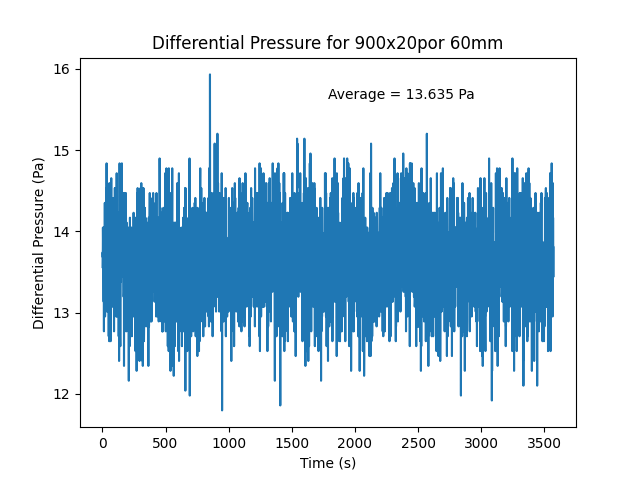
\includegraphics[width=0.75\textwidth]{900_20por_50-60_1hr_(.30-.45).png}
  \end{center}
  \caption{Differential pressure of a 6 cm, 900 pore, and 20 porosity 3-D printed porous 
material over an hour. The average differential pressure for the hour is displayed.}
  \label{fig:6cm_dp_graph}
\end{figure}

\begin{figure}[H]
  \begin{center}
    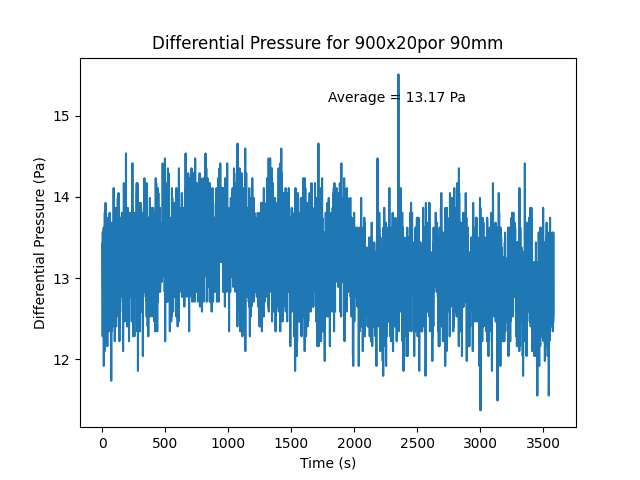
\includegraphics[width=0.75\textwidth]{900_20por_80-90(reprint)_1hr_(.25-.42speed).png}
  \end{center}
  \caption{Differential pressure of a 9 cm, 900 pore, and 20 porosity 3-D printed porous 
material over an hour. The average differential pressure for the hour is displayed.}
  \label{fig:9cm_dp_graph}
\end{figure}

\begin{figure}[H]
  \begin{center}
    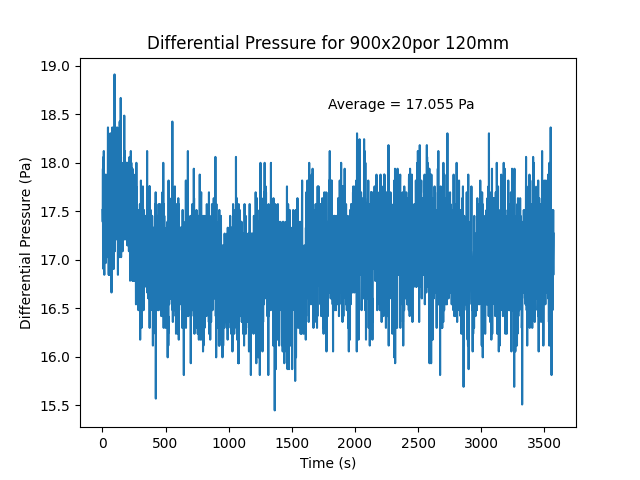
\includegraphics[width=0.75\textwidth]{900_20por_110-120_1hr_(.25-.42speed).png}
  \end{center}
  \caption{Differential pressure of a 12 cm, 900 pore, and 20 porosity 3-D printed porous 
material over an hour. The average differential pressure for the hour is displayed.}
  \label{fig:12cm_dp_graph}
\end{figure}
 
